\section{01 - Intro}

\begin{definition}{What's behind the Magic?} 
    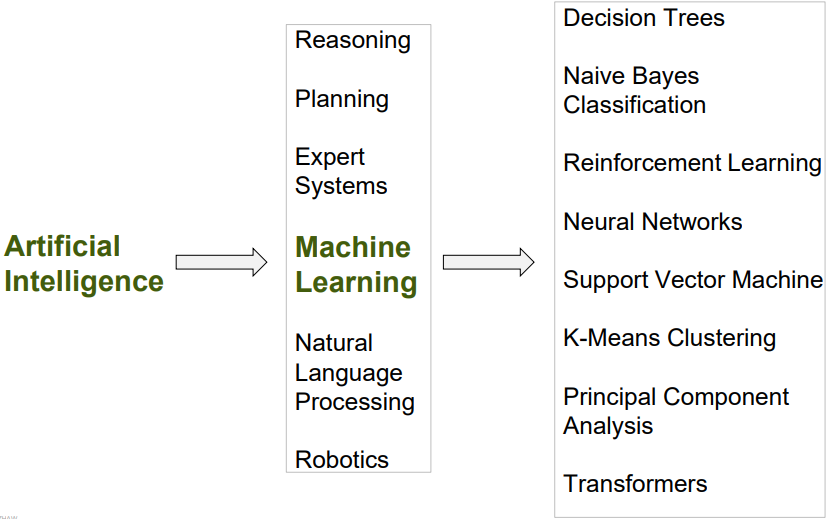
\includegraphics[width=\linewidth]{AI_magic.png}
\end{definition}

\begin{theorem}{Overview}

    \textcolor{frog}{textbf{Data Mining}}
    \begin{itemize}
        \item Discovering patterns in large data sets
        \item Extraction of patterns and knowledge from large amounts of data
    \end{itemize}

    \textcolor{frog}{textbf{Machine Learning}}
    \begin{itemize}
        \item Study of algorithms and statistical models without using explicit instructions, relying on patterns and inference instead
        \item Branch of AI devoted to developing and understanding methods that "learn", i.e. that leverage fata to make predictions or decisions (act like humans) without being explicity programmed to do so
    \end{itemize}

    \textcolor{blue}{textbf{Model}} is a logical, mathematical or probabilistic relationship between several variables

    \textcolor{blue}{textbf{Learning/Training}} in ML employs adaptive models, which are configured and parameterised based on the training data.

    \textcolor{frog}{textbf{Deep Learning}}
    \begin{itemize}
        \item Subset of machine learning where artificial neural networks (\textcolor{frog}{textbf{Deep Neural Networks}}), algorithms inspired by the human brain, learn from large amounts of data
        \item Uses multiple layers to progressively extract higher level features (attributes) from the raw input
    \end{itemize}

    \textcolor{frog}{textbf{Reinforcement Learning}} (Trial and Error)
    \begin{itemize}
        \item Concerned with how software agents take actions in an environment in order to maximize some notion of cumulative reward
    \end{itemize}

    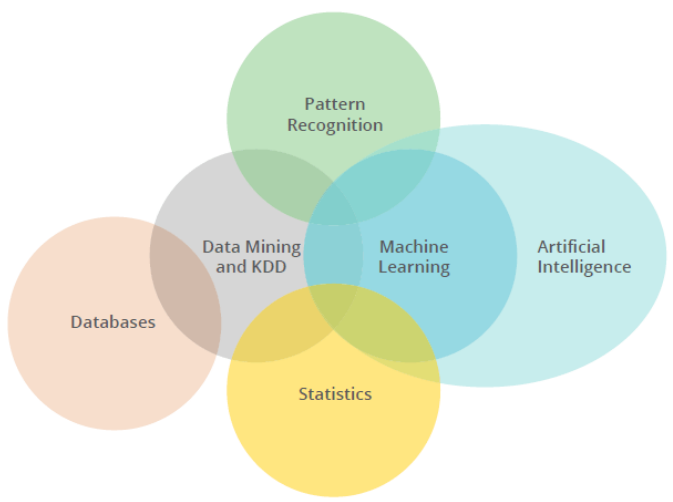
\includegraphics[width=\linewidth]{intro_overview.png}
\end{theorem}

\begin{concept}{Machine Learning - Types}

    \textcolor{darkturquoise}{\textbf{Supervised Learning}}
    \begin{itemize}
        \item The algorithm learns from labeled training data, and makes predictions (class, value) on unseen data
        \item Example: Classification, Regression
        \item see script for math shit
    \end{itemize}

    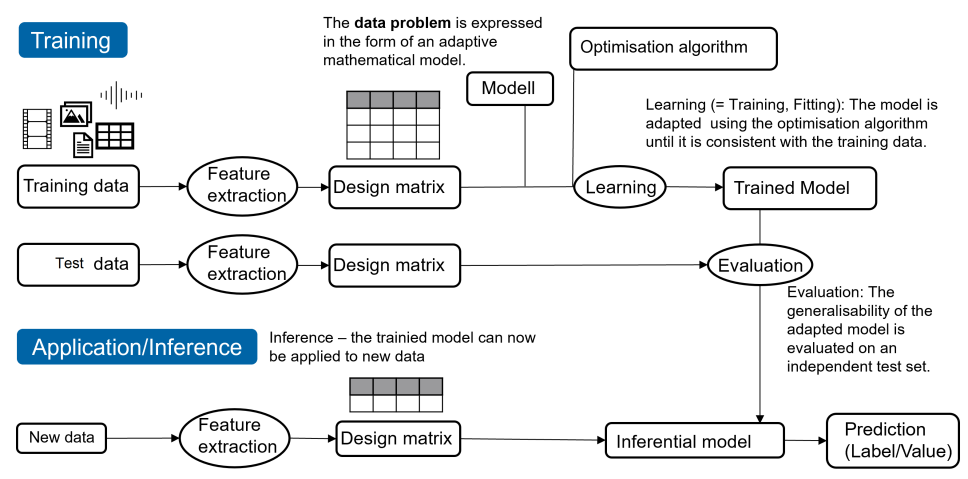
\includegraphics[width=\linewidth]{supervised_learning_pipeline.png}

    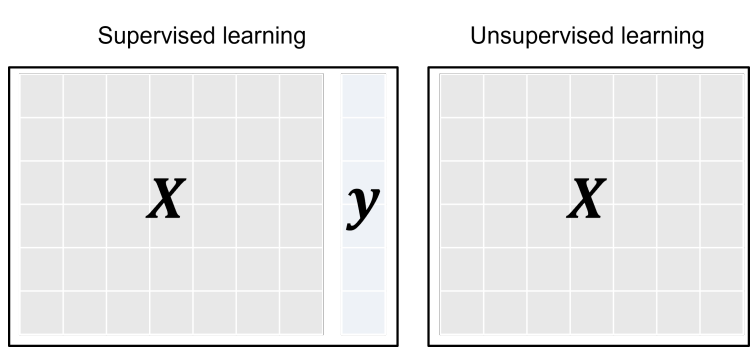
\includegraphics[width=\linewidth]{supervised_vs_unsupervised.png}

    \textcolor{darkturquoise}{\textbf{Unsupervised Learning}}
    \begin{itemize}
        \item The algorithm learns from unlabeled data, and determines data patterns / groupings / clusters
        \item Example: Clustering, Association, Hierarchical
    \end{itemize}

    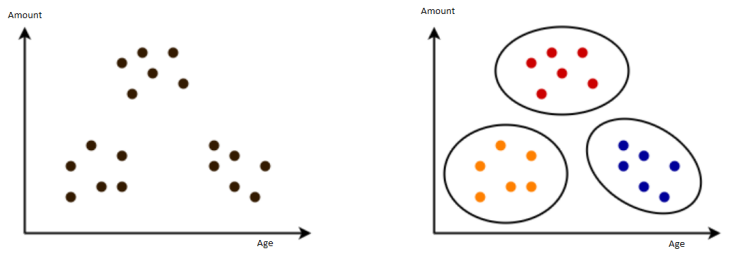
\includegraphics[width=\linewidth]{clustering_data.png}

    \textcolor{darkturquoise}{\textbf{Reinforcement Learning}}
    \begin{itemize}
        \item The algorithm learns to perform an action from experience
        \item Example: Game playing, Robotics
    \end{itemize}

    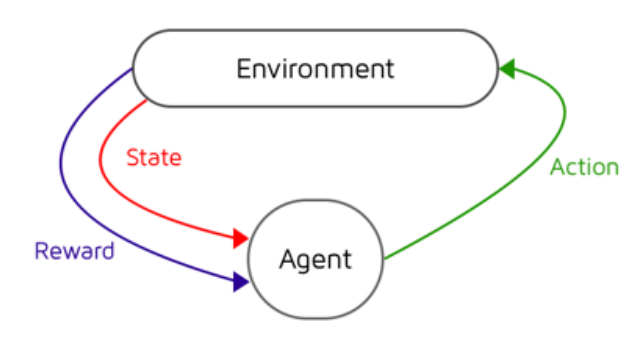
\includegraphics[width=\linewidth]{reinforcement_learning.png}
\end{concept}

\begin{definition}{Clustering}
    is the task of grouping a set of objects in such a way that objects in the same group (called a cluster) are more similar (in some sense) to each other than to
    those in other groups.
\end{definition}

\begin{definition}{Classification}
    is the problem of identifying to which of a set of categories a new observation belongs, on the basis of a training set of data containing observations (or instances) whose category membership is known. 
    E.g. correctly classifying (assigning a label to) an email as spam or not spam.

    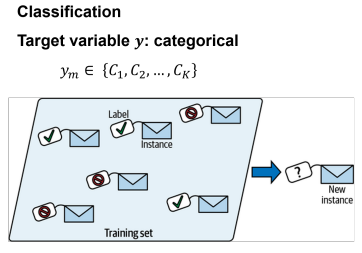
\includegraphics[width=\linewidth]{classification.png}
\end{definition}

\begin{definition}{Regression}
    is the problem of predicting and forecasting a concrete number based on a set of data containing observations whose category is known.

    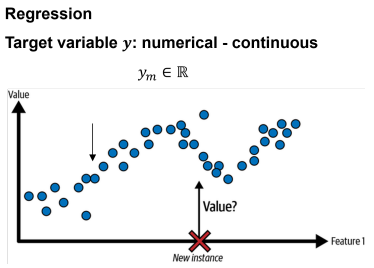
\includegraphics[width=\linewidth]{regression.png}
\end{definition}



